\section{Is Tantra dangerous?}

\begin{center}
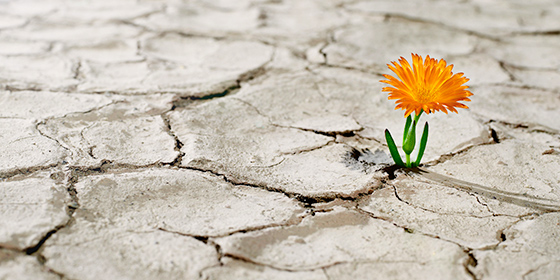
\includegraphics[width=7cm]{images/09_dangerous.jpg}
\end{center}

Whoever gets involved with Tantra is searching for something. How do we know that? Very easily: For the sake of using up time there are plenty of activities which are considerably less time-consuming, less effortful in energy, courage and patience than Tantra.

So what is the goal of this search? One thing that moves the most in the deepest way is the search for meaning, especially when in their personal history painful experiences  have happened. The search for making meaning of such experiences as well as of life itself can only be successful if we enlighten our dark spots, hidden in the shadows. If we bring light to those almost forgotten and carefully suppressed painful experiences.

That might not always feel like a stroll through a rose garden, which lies in the nature of things, and thus we can confidently agree here: Yes, Tantra is dangerous, as it endangers your whole past view on the world!

I remember a participant about the age of sixty. She took part in a short entry-level retreat and courageously stayed until the very end, even though she obviously had to struggle with intense emotions. Afterwards she came to me and said: "You know, it's all nice and good here, but I think I would rather not wake up those sleeping dogs."

That's a valid and conscious decision: I prefer to keep my view on things. The effort to gain a new, probably more relaxed worldview is too scary for me for now. Yet, once you have determined to bring up the light out of the depth, then it is rather irrelevant what you do. You can even attend a plain painting course: Something you experience there will bring the burdensome experience from the past to the surface of your consciousness, so it can be dissolved.

That's also what Western Tantra does, just with caution and focus and with the support of thoroughly and extensively educated facilitators.

Does it also happen that someone seriously "freaks out" - due to an intense contact with an emotional burden of the past - and is not able to help himself or herself anymore? Indeed, it does. No effective method can guarantee harmlessness. But we had to intercept such a situation only a few times within the last 25 years. For such moments, good facilitators offer competent and empathetic support in the process, during the retreat and also afterwards if requested.

Tantra uses an approach which carefully reveals old and deeply hidden things.That's why there is so much astonishing feedback of therapy-experienced participants. They cannot believe that even after a single retreat they have progressed so much more than in many years of conventional therapy. However, their previous effort is never in vain. Often it is exactly due to a past therapy that they can get unexpected and quick results.

To sum it up, is Tantra  dangerous? Absolutely!

Your destructive thought convictions, rigid patterns, less than helpful habits and all the other elements which prevent you from reaching your highest potential may already be scared.
